\documentclass{extbook}[14pt]
\usepackage{multicol, enumerate, enumitem, hyperref, color, soul, setspace, parskip, fancyhdr, amssymb, amsthm, amsmath, latexsym, units, mathtools}
\everymath{\displaystyle}
\usepackage[headsep=0.5cm,headheight=0cm, left=1 in,right= 1 in,top= 1 in,bottom= 1 in]{geometry}
\usepackage{dashrule}  % Package to use the command below to create lines between items
\newcommand{\litem}[1]{\item #1

\rule{\textwidth}{0.4pt}}
\pagestyle{fancy}
\lhead{}
\chead{Answer Key for Makeup Progress Quiz 3 Version ALL}
\rhead{}
\lfoot{1648-1753}
\cfoot{}
\rfoot{Summer C 2021}
\begin{document}
\textbf{This key should allow you to understand why you choose the option you did (beyond just getting a question right or wrong). \href{https://xronos.clas.ufl.edu/mac1105spring2020/courseDescriptionAndMisc/Exams/LearningFromResults}{More instructions on how to use this key can be found here}.}

\textbf{If you have a suggestion to make the keys better, \href{https://forms.gle/CZkbZmPbC9XALEE88}{please fill out the short survey here}.}

\textit{Note: This key is auto-generated and may contain issues and/or errors. The keys are reviewed after each exam to ensure grading is done accurately. If there are issues (like duplicate options), they are noted in the offline gradebook. The keys are a work-in-progress to give students as many resources to improve as possible.}

\rule{\textwidth}{0.4pt}

\begin{enumerate}\litem{
Construct the lowest-degree polynomial given the zeros below. Then, choose the intervals that contain the coefficients of the polynomial in the form $x^3+bx^2+cx+d$.
\[ 3 - 2 i \text{ and } -3 \]The solution is \( x^{3} -3 x^{2} -5 x + 39 \), which is option D.\begin{enumerate}[label=\Alph*.]
\item \( b \in [1.1, 4], c \in [-5.1, -3.6], \text{ and } d \in [-40, -32] \)

$x^{3} +3 x^{2} -5 x -39$, which corresponds to multiplying out $(x-(3 - 2 i))(x-(3 + 2 i))(x -3)$.
\item \( b \in [-0.4, 2], c \in [-2.9, 0.1], \text{ and } d \in [-9, -4] \)

$x^{3} + x^{2} -9$, which corresponds to multiplying out $(x -3)(x + 3)$.
\item \( b \in [-0.4, 2], c \in [3.2, 8.7], \text{ and } d \in [4, 7] \)

$x^{3} + x^{2} +5 x + 6$, which corresponds to multiplying out $(x + 2)(x + 3)$.
\item \( b \in [-6.7, -1], c \in [-5.1, -3.6], \text{ and } d \in [36, 41] \)

* $x^{3} -3 x^{2} -5 x + 39$, which is the correct option.
\item \( \text{None of the above.} \)

This corresponds to making an unanticipated error or not understanding how to use nonreal complex numbers to create the lowest-degree polynomial. If you chose this and are not sure what you did wrong, please contact the coordinator for help.
\end{enumerate}

\textbf{General Comment:} Remember that the conjugate of $a+bi$ is $a-bi$. Since these zeros always come in pairs, we need to multiply out $(x-(3 - 2 i))(x-(3 + 2 i))(x-(-3))$.
}
\litem{
Describe the end behavior of the polynomial below.
\[ f(x) = 2(x - 9)^{3}(x + 9)^{8}(x - 7)^{3}(x + 7)^{5} \]The solution is the graph below, which is option D.
    \begin{center}
        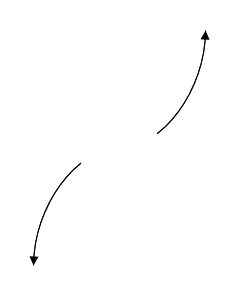
\includegraphics[width=0.3\textwidth]{../Figures/polyEndBehaviorDA.png}
    \end{center}\begin{enumerate}[label=\Alph*.]
\begin{multicols}{2}
\item 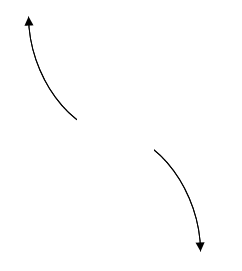
\includegraphics[width = 0.3\textwidth]{../Figures/polyEndBehaviorAA.png}
\item 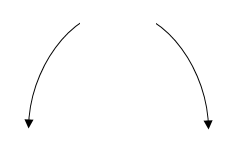
\includegraphics[width = 0.3\textwidth]{../Figures/polyEndBehaviorBA.png}
\item 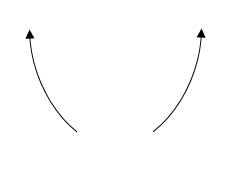
\includegraphics[width = 0.3\textwidth]{../Figures/polyEndBehaviorCA.png}
\item 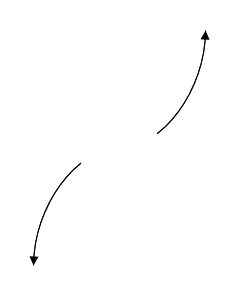
\includegraphics[width = 0.3\textwidth]{../Figures/polyEndBehaviorDA.png}
\end{multicols}\item None of the above.\end{enumerate}
\textbf{General Comment:} Remember that end behavior is determined by the leading coefficient AND whether the \textbf{sum} of the multiplicities is positive or negative.
}
\litem{
Describe the end behavior of the polynomial below.
\[ f(x) = -4(x - 2)^{5}(x + 2)^{10}(x - 3)^{5}(x + 3)^{6} \]The solution is the graph below, which is option B.
    \begin{center}
        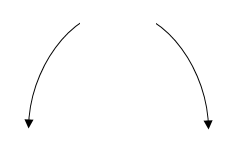
\includegraphics[width=0.3\textwidth]{../Figures/polyEndBehaviorCopyBA.png}
    \end{center}\begin{enumerate}[label=\Alph*.]
\begin{multicols}{2}
\item 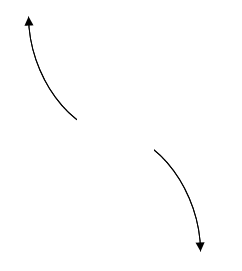
\includegraphics[width = 0.3\textwidth]{../Figures/polyEndBehaviorCopyAA.png}
\item 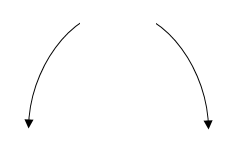
\includegraphics[width = 0.3\textwidth]{../Figures/polyEndBehaviorCopyBA.png}
\item 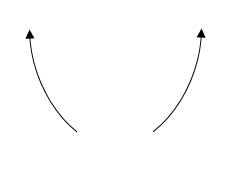
\includegraphics[width = 0.3\textwidth]{../Figures/polyEndBehaviorCopyCA.png}
\item 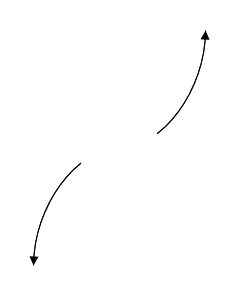
\includegraphics[width = 0.3\textwidth]{../Figures/polyEndBehaviorCopyDA.png}
\end{multicols}\item None of the above.\end{enumerate}
\textbf{General Comment:} Remember that end behavior is determined by the leading coefficient AND whether the \textbf{sum} of the multiplicities is positive or negative.
}
\litem{
Construct the lowest-degree polynomial given the zeros below. Then, choose the intervals that contain the coefficients of the polynomial in the form $ax^3+bx^2+cx+d$.
\[ -6, \frac{-3}{4}, \text{ and } \frac{7}{2} \]The solution is \( 8x^{3} +26 x^{2} -153 x -126 \), which is option C.\begin{enumerate}[label=\Alph*.]
\item \( a \in [3, 10], b \in [-75, -66], c \in [108, 118], \text{ and } d \in [125, 128] \)

$8x^{3} -70 x^{2} +111 x + 126$, which corresponds to multiplying out $(x -6)(4x + 3)(2x -7)$.
\item \( a \in [3, 10], b \in [-26, -24], c \in [-154, -145], \text{ and } d \in [125, 128] \)

$8x^{3} -26 x^{2} -153 x + 126$, which corresponds to multiplying out $(x -6)(4x -3)(2x + 7)$.
\item \( a \in [3, 10], b \in [23, 33], c \in [-154, -145], \text{ and } d \in [-130, -119] \)

* $8x^{3} +26 x^{2} -153 x -126$, which is the correct option.
\item \( a \in [3, 10], b \in [-89, -77], c \in [222, 233], \text{ and } d \in [-130, -119] \)

$8x^{3} -82 x^{2} +225 x -126$, which corresponds to multiplying out $(x -6)(4x -3)(2x -7)$.
\item \( a \in [3, 10], b \in [23, 33], c \in [-154, -145], \text{ and } d \in [125, 128] \)

$8x^{3} +26 x^{2} -153 x + 126$, which corresponds to multiplying everything correctly except the constant term.
\end{enumerate}

\textbf{General Comment:} To construct the lowest-degree polynomial, you want to multiply out $(x + 6)(4x + 3)(2x -7)$
}
\litem{
Describe the zero behavior of the zero $x = 3$ of the polynomial below.
\[ f(x) = 6(x - 3)^{4}(x + 3)^{9}(x + 7)^{4}(x - 7)^{8} \]The solution is the graph below, which is option C.
    \begin{center}
        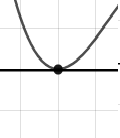
\includegraphics[width=0.3\textwidth]{../Figures/polyZeroBehaviorCA.png}
    \end{center}\begin{enumerate}[label=\Alph*.]
\begin{multicols}{2}
\item 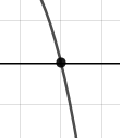
\includegraphics[width = 0.3\textwidth]{../Figures/polyZeroBehaviorAA.png}
\item 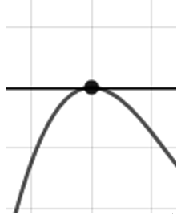
\includegraphics[width = 0.3\textwidth]{../Figures/polyZeroBehaviorBA.png}
\item 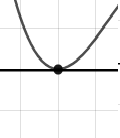
\includegraphics[width = 0.3\textwidth]{../Figures/polyZeroBehaviorCA.png}
\item 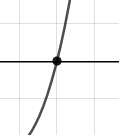
\includegraphics[width = 0.3\textwidth]{../Figures/polyZeroBehaviorDA.png}
\end{multicols}\item None of the above.\end{enumerate}
\textbf{General Comment:} You will need to sketch the entire graph, then zoom in on the zero the question asks about.
}
\litem{
Which of the following equations \textit{could} be of the graph presented below?

\begin{center}
    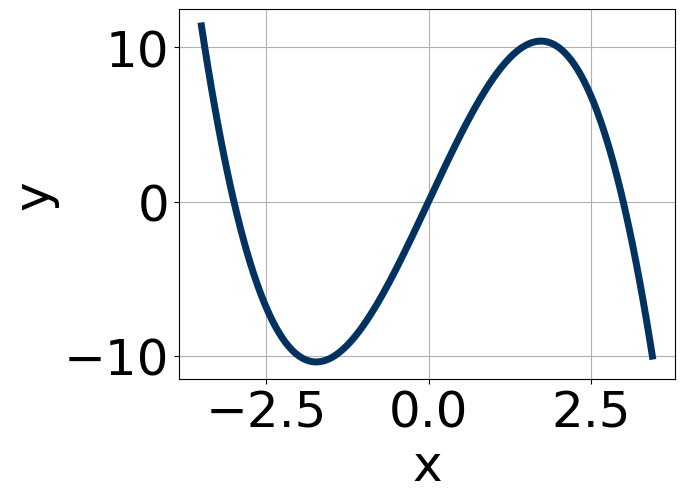
\includegraphics[width=0.5\textwidth]{../Figures/polyGraphToFunctionA.png}
\end{center}


The solution is \( -14x^{11} (x - 3)^{5} (x + 3)^{9} \), which is option C.\begin{enumerate}[label=\Alph*.]
\item \( 5x^{5} (x - 3)^{10} (x + 3)^{5} \)

The factor $(x - 3)$ should have an odd power and the leading coefficient should be the opposite sign.
\item \( -7x^{9} (x - 3)^{4} (x + 3)^{9} \)

The factor $3$ should have been an odd power.
\item \( -14x^{11} (x - 3)^{5} (x + 3)^{9} \)

* This is the correct option.
\item \( -18x^{9} (x - 3)^{4} (x + 3)^{8} \)

The factors $3$ and $-3$ have have been odd power.
\item \( 17x^{7} (x - 3)^{5} (x + 3)^{5} \)

This corresponds to the leading coefficient being the opposite value than it should be.
\end{enumerate}

\textbf{General Comment:} General Comments: Draw the x-axis to determine which zeros are touching (and so have even multiplicity) or cross (and have odd multiplicity).
}
\litem{
Construct the lowest-degree polynomial given the zeros below. Then, choose the intervals that contain the coefficients of the polynomial in the form $x^3+bx^2+cx+d$.
\[ -2 - 5 i \text{ and } 3 \]The solution is \( x^{3} + x^{2} +17 x -87 \), which is option A.\begin{enumerate}[label=\Alph*.]
\item \( b \in [0.2, 3.8], c \in [16.8, 19.7], \text{ and } d \in [-92, -81] \)

* $x^{3} + x^{2} +17 x -87$, which is the correct option.
\item \( b \in [0.2, 3.8], c \in [-3.5, 0.3], \text{ and } d \in [-9, -3] \)

$x^{3} + x^{2} -x -6$, which corresponds to multiplying out $(x + 2)(x -3)$.
\item \( b \in [-4.5, 0.5], c \in [16.8, 19.7], \text{ and } d \in [86, 92] \)

$x^{3} -1 x^{2} +17 x + 87$, which corresponds to multiplying out $(x-(-2 - 5 i))(x-(-2 + 5 i))(x + 3)$.
\item \( b \in [0.2, 3.8], c \in [1.8, 4.3], \text{ and } d \in [-18, -11] \)

$x^{3} + x^{2} +2 x -15$, which corresponds to multiplying out $(x + 5)(x -3)$.
\item \( \text{None of the above.} \)

This corresponds to making an unanticipated error or not understanding how to use nonreal complex numbers to create the lowest-degree polynomial. If you chose this and are not sure what you did wrong, please contact the coordinator for help.
\end{enumerate}

\textbf{General Comment:} Remember that the conjugate of $a+bi$ is $a-bi$. Since these zeros always come in pairs, we need to multiply out $(x-(-2 - 5 i))(x-(-2 + 5 i))(x-(3))$.
}
\litem{
Describe the zero behavior of the zero $x = 5$ of the polynomial below.
\[ f(x) = -9(x - 6)^{11}(x + 6)^{9}(x - 5)^{7}(x + 5)^{6} \]The solution is the graph below, which is option D.
    \begin{center}
        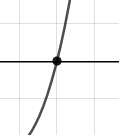
\includegraphics[width=0.3\textwidth]{../Figures/polyZeroBehaviorCopyDA.png}
    \end{center}\begin{enumerate}[label=\Alph*.]
\begin{multicols}{2}
\item 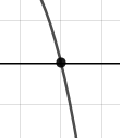
\includegraphics[width = 0.3\textwidth]{../Figures/polyZeroBehaviorCopyAA.png}
\item 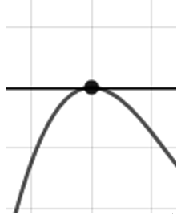
\includegraphics[width = 0.3\textwidth]{../Figures/polyZeroBehaviorCopyBA.png}
\item 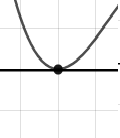
\includegraphics[width = 0.3\textwidth]{../Figures/polyZeroBehaviorCopyCA.png}
\item 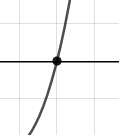
\includegraphics[width = 0.3\textwidth]{../Figures/polyZeroBehaviorCopyDA.png}
\end{multicols}\item None of the above.\end{enumerate}
\textbf{General Comment:} You will need to sketch the entire graph, then zoom in on the zero the question asks about.
}
\litem{
Construct the lowest-degree polynomial given the zeros below. Then, choose the intervals that contain the coefficients of the polynomial in the form $ax^3+bx^2+cx+d$.
\[ \frac{5}{3}, 7, \text{ and } \frac{-7}{5} \]The solution is \( 15x^{3} -109 x^{2} -7 x + 245 \), which is option B.\begin{enumerate}[label=\Alph*.]
\item \( a \in [13, 24], b \in [143, 153], c \in [348, 358], \text{ and } d \in [239, 253] \)

$15x^{3} +151 x^{2} +357 x + 245$, which corresponds to multiplying out $(3x + 5)(x + 7)(5x + 7)$.
\item \( a \in [13, 24], b \in [-110, -101], c \in [-10, -4], \text{ and } d \in [239, 253] \)

* $15x^{3} -109 x^{2} -7 x + 245$, which is the correct option.
\item \( a \in [13, 24], b \in [-110, -101], c \in [-10, -4], \text{ and } d \in [-247, -238] \)

$15x^{3} -109 x^{2} -7 x -245$, which corresponds to multiplying everything correctly except the constant term.
\item \( a \in [13, 24], b \in [106, 114], c \in [-10, -4], \text{ and } d \in [-247, -238] \)

$15x^{3} +109 x^{2} -7 x -245$, which corresponds to multiplying out $(3x + 5)(x + 7)(5x -7)$.
\item \( a \in [13, 24], b \in [-60, -56], c \in [-287, -277], \text{ and } d \in [-247, -238] \)

$15x^{3} -59 x^{2} -287 x -245$, which corresponds to multiplying out $(3x + 5)(x -7)(5x + 7)$.
\end{enumerate}

\textbf{General Comment:} To construct the lowest-degree polynomial, you want to multiply out $(3x -5)(x -7)(5x + 7)$
}
\litem{
Which of the following equations \textit{could} be of the graph presented below?

\begin{center}
    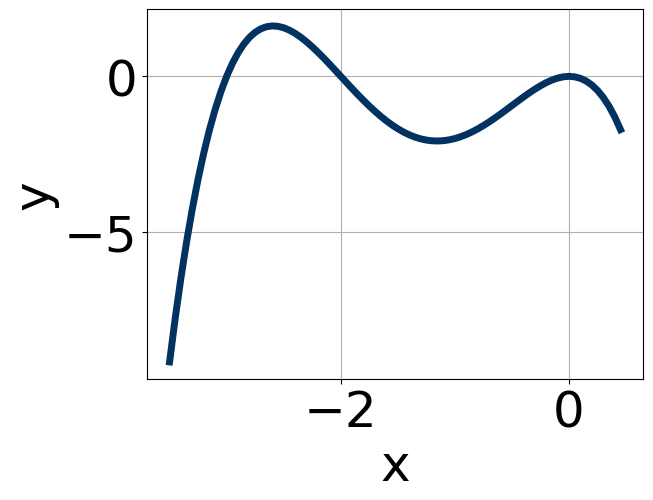
\includegraphics[width=0.5\textwidth]{../Figures/polyGraphToFunctionCopyA.png}
\end{center}


The solution is \( -18x^{6} (x + 3)^{11} (x + 2)^{9} \), which is option E.\begin{enumerate}[label=\Alph*.]
\item \( 9x^{4} (x + 3)^{7} (x + 2)^{11} \)

This corresponds to the leading coefficient being the opposite value than it should be.
\item \( -20x^{10} (x + 3)^{10} (x + 2)^{11} \)

The factor $(x + 3)$ should have an odd power.
\item \( 14x^{4} (x + 3)^{9} (x + 2)^{8} \)

The factor $(x + 2)$ should have an odd power and the leading coefficient should be the opposite sign.
\item \( -13x^{9} (x + 3)^{6} (x + 2)^{9} \)

The factor $0$ should have an even power and the factor $-3$ should have an odd power.
\item \( -18x^{6} (x + 3)^{11} (x + 2)^{9} \)

* This is the correct option.
\end{enumerate}

\textbf{General Comment:} General Comments: Draw the x-axis to determine which zeros are touching (and so have even multiplicity) or cross (and have odd multiplicity).
}
\litem{
Construct the lowest-degree polynomial given the zeros below. Then, choose the intervals that contain the coefficients of the polynomial in the form $x^3+bx^2+cx+d$.
\[ 5 - 3 i \text{ and } 2 \]The solution is \( x^{3} -12 x^{2} +54 x -68 \), which is option C.\begin{enumerate}[label=\Alph*.]
\item \( b \in [-9, 6], c \in [0, 6], \text{ and } d \in [-9, 1] \)

$x^{3} + x^{2} +x -6$, which corresponds to multiplying out $(x + 3)(x -2)$.
\item \( b \in [10, 13], c \in [52, 62], \text{ and } d \in [68, 76] \)

$x^{3} +12 x^{2} +54 x + 68$, which corresponds to multiplying out $(x-(5 - 3 i))(x-(5 + 3 i))(x + 2)$.
\item \( b \in [-14, -11], c \in [52, 62], \text{ and } d \in [-76, -62] \)

* $x^{3} -12 x^{2} +54 x -68$, which is the correct option.
\item \( b \in [-9, 6], c \in [-13, -1], \text{ and } d \in [4, 16] \)

$x^{3} + x^{2} -7 x + 10$, which corresponds to multiplying out $(x -5)(x -2)$.
\item \( \text{None of the above.} \)

This corresponds to making an unanticipated error or not understanding how to use nonreal complex numbers to create the lowest-degree polynomial. If you chose this and are not sure what you did wrong, please contact the coordinator for help.
\end{enumerate}

\textbf{General Comment:} Remember that the conjugate of $a+bi$ is $a-bi$. Since these zeros always come in pairs, we need to multiply out $(x-(5 - 3 i))(x-(5 + 3 i))(x-(2))$.
}
\litem{
Describe the end behavior of the polynomial below.
\[ f(x) = 8(x + 3)^{3}(x - 3)^{8}(x - 2)^{3}(x + 2)^{4} \]The solution is the graph below, which is option C.
    \begin{center}
        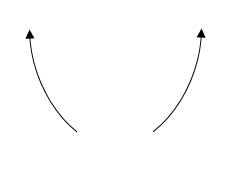
\includegraphics[width=0.3\textwidth]{../Figures/polyEndBehaviorCB.png}
    \end{center}\begin{enumerate}[label=\Alph*.]
\begin{multicols}{2}
\item 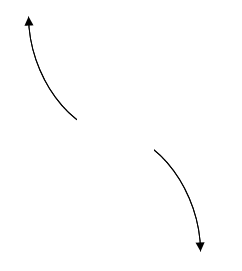
\includegraphics[width = 0.3\textwidth]{../Figures/polyEndBehaviorAB.png}
\item 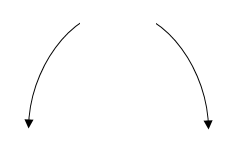
\includegraphics[width = 0.3\textwidth]{../Figures/polyEndBehaviorBB.png}
\item 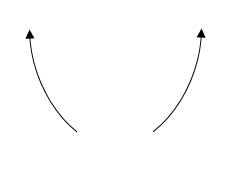
\includegraphics[width = 0.3\textwidth]{../Figures/polyEndBehaviorCB.png}
\item 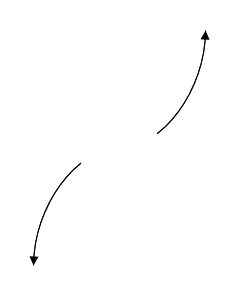
\includegraphics[width = 0.3\textwidth]{../Figures/polyEndBehaviorDB.png}
\end{multicols}\item None of the above.\end{enumerate}
\textbf{General Comment:} Remember that end behavior is determined by the leading coefficient AND whether the \textbf{sum} of the multiplicities is positive or negative.
}
\litem{
Describe the end behavior of the polynomial below.
\[ f(x) = 7(x - 4)^{4}(x + 4)^{5}(x + 3)^{3}(x - 3)^{5} \]The solution is the graph below, which is option D.
    \begin{center}
        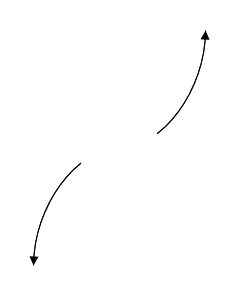
\includegraphics[width=0.3\textwidth]{../Figures/polyEndBehaviorCopyDB.png}
    \end{center}\begin{enumerate}[label=\Alph*.]
\begin{multicols}{2}
\item 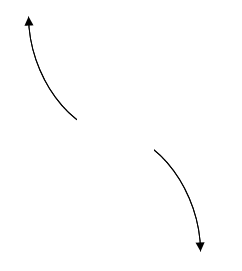
\includegraphics[width = 0.3\textwidth]{../Figures/polyEndBehaviorCopyAB.png}
\item 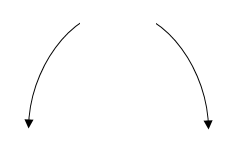
\includegraphics[width = 0.3\textwidth]{../Figures/polyEndBehaviorCopyBB.png}
\item 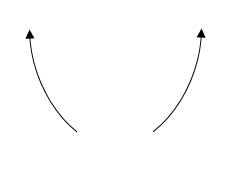
\includegraphics[width = 0.3\textwidth]{../Figures/polyEndBehaviorCopyCB.png}
\item 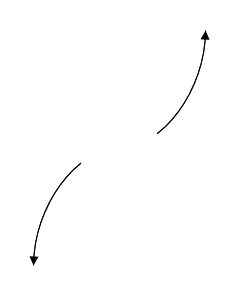
\includegraphics[width = 0.3\textwidth]{../Figures/polyEndBehaviorCopyDB.png}
\end{multicols}\item None of the above.\end{enumerate}
\textbf{General Comment:} Remember that end behavior is determined by the leading coefficient AND whether the \textbf{sum} of the multiplicities is positive or negative.
}
\litem{
Construct the lowest-degree polynomial given the zeros below. Then, choose the intervals that contain the coefficients of the polynomial in the form $ax^3+bx^2+cx+d$.
\[ 7, \frac{-1}{5}, \text{ and } \frac{2}{3} \]The solution is \( 15x^{3} -112 x^{2} +47 x + 14 \), which is option C.\begin{enumerate}[label=\Alph*.]
\item \( a \in [15, 17], b \in [110.6, 112.3], c \in [44, 57], \text{ and } d \in [-17, -12] \)

$15x^{3} +112 x^{2} +47 x -14$, which corresponds to multiplying out $(x + 7)(5x -1)(3x + 2)$.
\item \( a \in [15, 17], b \in [91.8, 95.9], c \in [-92, -82], \text{ and } d \in [14, 19] \)

$15x^{3} +92 x^{2} -89 x + 14$, which corresponds to multiplying out $(x + 7)(5x -1)(3x -2)$.
\item \( a \in [15, 17], b \in [-112.5, -108.4], c \in [44, 57], \text{ and } d \in [14, 19] \)

* $15x^{3} -112 x^{2} +47 x + 14$, which is the correct option.
\item \( a \in [15, 17], b \in [96, 100.8], c \in [-52, -44], \text{ and } d \in [-17, -12] \)

$15x^{3} +98 x^{2} -51 x -14$, which corresponds to multiplying out $(x + 7)(5x + 1)(3x -2)$.
\item \( a \in [15, 17], b \in [-112.5, -108.4], c \in [44, 57], \text{ and } d \in [-17, -12] \)

$15x^{3} -112 x^{2} +47 x -14$, which corresponds to multiplying everything correctly except the constant term.
\end{enumerate}

\textbf{General Comment:} To construct the lowest-degree polynomial, you want to multiply out $(x -7)(5x + 1)(3x -2)$
}
\litem{
Describe the zero behavior of the zero $x = 2$ of the polynomial below.
\[ f(x) = -3(x + 2)^{4}(x - 2)^{5}(x - 7)^{5}(x + 7)^{7} \]The solution is the graph below, which is option D.
    \begin{center}
        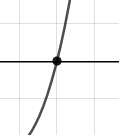
\includegraphics[width=0.3\textwidth]{../Figures/polyZeroBehaviorDB.png}
    \end{center}\begin{enumerate}[label=\Alph*.]
\begin{multicols}{2}
\item 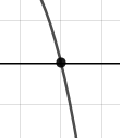
\includegraphics[width = 0.3\textwidth]{../Figures/polyZeroBehaviorAB.png}
\item 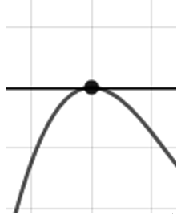
\includegraphics[width = 0.3\textwidth]{../Figures/polyZeroBehaviorBB.png}
\item 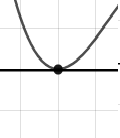
\includegraphics[width = 0.3\textwidth]{../Figures/polyZeroBehaviorCB.png}
\item 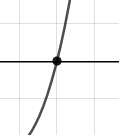
\includegraphics[width = 0.3\textwidth]{../Figures/polyZeroBehaviorDB.png}
\end{multicols}\item None of the above.\end{enumerate}
\textbf{General Comment:} You will need to sketch the entire graph, then zoom in on the zero the question asks about.
}
\litem{
Which of the following equations \textit{could} be of the graph presented below?

\begin{center}
    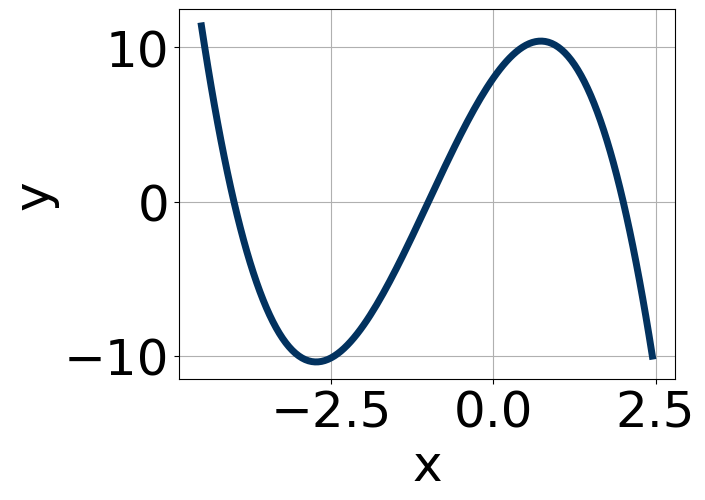
\includegraphics[width=0.5\textwidth]{../Figures/polyGraphToFunctionB.png}
\end{center}


The solution is \( -10(x - 2)^{5} (x + 4)^{7} (x + 1)^{11} \), which is option E.\begin{enumerate}[label=\Alph*.]
\item \( -8(x - 2)^{10} (x + 4)^{6} (x + 1)^{5} \)

The factors $2$ and $-4$ have have been odd power.
\item \( 12(x - 2)^{8} (x + 4)^{7} (x + 1)^{7} \)

The factor $(x - 2)$ should have an odd power and the leading coefficient should be the opposite sign.
\item \( -4(x - 2)^{10} (x + 4)^{11} (x + 1)^{11} \)

The factor $2$ should have been an odd power.
\item \( 11(x - 2)^{7} (x + 4)^{9} (x + 1)^{9} \)

This corresponds to the leading coefficient being the opposite value than it should be.
\item \( -10(x - 2)^{5} (x + 4)^{7} (x + 1)^{11} \)

* This is the correct option.
\end{enumerate}

\textbf{General Comment:} General Comments: Draw the x-axis to determine which zeros are touching (and so have even multiplicity) or cross (and have odd multiplicity).
}
\litem{
Construct the lowest-degree polynomial given the zeros below. Then, choose the intervals that contain the coefficients of the polynomial in the form $x^3+bx^2+cx+d$.
\[ 4 + 5 i \text{ and } 1 \]The solution is \( x^{3} -9 x^{2} +49 x -41 \), which is option A.\begin{enumerate}[label=\Alph*.]
\item \( b \in [-11, -5], c \in [48.79, 49.11], \text{ and } d \in [-41.09, -39.64] \)

* $x^{3} -9 x^{2} +49 x -41$, which is the correct option.
\item \( b \in [1, 6], c \in [-5.16, -3.28], \text{ and } d \in [2.13, 4.62] \)

$x^{3} + x^{2} -5 x + 4$, which corresponds to multiplying out $(x -4)(x -1)$.
\item \( b \in [1, 6], c \in [-6.36, -5.54], \text{ and } d \in [4.44, 5.18] \)

$x^{3} + x^{2} -6 x + 5$, which corresponds to multiplying out $(x -5)(x -1)$.
\item \( b \in [3, 14], c \in [48.79, 49.11], \text{ and } d \in [39.48, 43] \)

$x^{3} +9 x^{2} +49 x + 41$, which corresponds to multiplying out $(x-(4 + 5 i))(x-(4 - 5 i))(x + 1)$.
\item \( \text{None of the above.} \)

This corresponds to making an unanticipated error or not understanding how to use nonreal complex numbers to create the lowest-degree polynomial. If you chose this and are not sure what you did wrong, please contact the coordinator for help.
\end{enumerate}

\textbf{General Comment:} Remember that the conjugate of $a+bi$ is $a-bi$. Since these zeros always come in pairs, we need to multiply out $(x-(4 + 5 i))(x-(4 - 5 i))(x-(1))$.
}
\litem{
Describe the zero behavior of the zero $x = -7$ of the polynomial below.
\[ f(x) = -9(x - 4)^{5}(x + 4)^{2}(x + 7)^{11}(x - 7)^{8} \]The solution is the graph below, which is option D.
    \begin{center}
        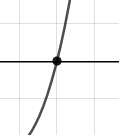
\includegraphics[width=0.3\textwidth]{../Figures/polyZeroBehaviorCopyDB.png}
    \end{center}\begin{enumerate}[label=\Alph*.]
\begin{multicols}{2}
\item 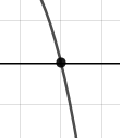
\includegraphics[width = 0.3\textwidth]{../Figures/polyZeroBehaviorCopyAB.png}
\item 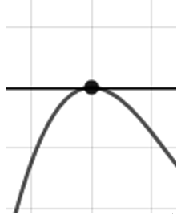
\includegraphics[width = 0.3\textwidth]{../Figures/polyZeroBehaviorCopyBB.png}
\item 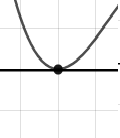
\includegraphics[width = 0.3\textwidth]{../Figures/polyZeroBehaviorCopyCB.png}
\item 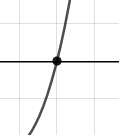
\includegraphics[width = 0.3\textwidth]{../Figures/polyZeroBehaviorCopyDB.png}
\end{multicols}\item None of the above.\end{enumerate}
\textbf{General Comment:} You will need to sketch the entire graph, then zoom in on the zero the question asks about.
}
\litem{
Construct the lowest-degree polynomial given the zeros below. Then, choose the intervals that contain the coefficients of the polynomial in the form $ax^3+bx^2+cx+d$.
\[ -1, \frac{-4}{5}, \text{ and } \frac{3}{5} \]The solution is \( 25x^{3} +30 x^{2} -7 x -12 \), which is option D.\begin{enumerate}[label=\Alph*.]
\item \( a \in [19, 32], b \in [28, 33], c \in [-10, -3], \text{ and } d \in [12, 19] \)

$25x^{3} +30 x^{2} -7 x + 12$, which corresponds to multiplying everything correctly except the constant term.
\item \( a \in [19, 32], b \in [-26, -18], c \in [-20, -16], \text{ and } d \in [12, 19] \)

$25x^{3} -20 x^{2} -17 x + 12$, which corresponds to multiplying out $(x -1)(5x + 4)(5x -3)$.
\item \( a \in [19, 32], b \in [-64, -56], c \in [45, 49], \text{ and } d \in [-12, -9] \)

$25x^{3} -60 x^{2} +47 x -12$, which corresponds to multiplying out $(x -1)(5x -4)(5x -3)$.
\item \( a \in [19, 32], b \in [28, 33], c \in [-10, -3], \text{ and } d \in [-12, -9] \)

* $25x^{3} +30 x^{2} -7 x -12$, which is the correct option.
\item \( a \in [19, 32], b \in [-32, -26], c \in [-10, -3], \text{ and } d \in [12, 19] \)

$25x^{3} -30 x^{2} -7 x + 12$, which corresponds to multiplying out $(x -1)(5x -4)(5x + 3)$.
\end{enumerate}

\textbf{General Comment:} To construct the lowest-degree polynomial, you want to multiply out $(x + 1)(5x + 4)(5x -3)$
}
\litem{
Which of the following equations \textit{could} be of the graph presented below?

\begin{center}
    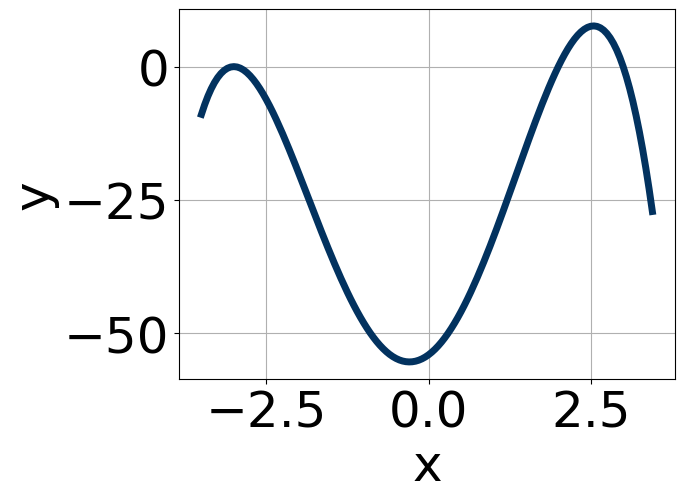
\includegraphics[width=0.5\textwidth]{../Figures/polyGraphToFunctionCopyB.png}
\end{center}


The solution is \( -5(x + 3)^{6} (x - 2)^{5} (x - 3)^{9} \), which is option E.\begin{enumerate}[label=\Alph*.]
\item \( 12(x + 3)^{8} (x - 2)^{11} (x - 3)^{9} \)

This corresponds to the leading coefficient being the opposite value than it should be.
\item \( -19(x + 3)^{6} (x - 2)^{10} (x - 3)^{11} \)

The factor $(x - 2)$ should have an odd power.
\item \( -20(x + 3)^{9} (x - 2)^{6} (x - 3)^{9} \)

The factor $-3$ should have an even power and the factor $2$ should have an odd power.
\item \( 6(x + 3)^{4} (x - 2)^{11} (x - 3)^{4} \)

The factor $(x - 3)$ should have an odd power and the leading coefficient should be the opposite sign.
\item \( -5(x + 3)^{6} (x - 2)^{5} (x - 3)^{9} \)

* This is the correct option.
\end{enumerate}

\textbf{General Comment:} General Comments: Draw the x-axis to determine which zeros are touching (and so have even multiplicity) or cross (and have odd multiplicity).
}
\litem{
Construct the lowest-degree polynomial given the zeros below. Then, choose the intervals that contain the coefficients of the polynomial in the form $x^3+bx^2+cx+d$.
\[ 5 + 2 i \text{ and } 1 \]The solution is \( x^{3} -11 x^{2} +39 x -29 \), which is option A.\begin{enumerate}[label=\Alph*.]
\item \( b \in [-18, -7], c \in [35.4, 40.7], \text{ and } d \in [-30.8, -28.8] \)

* $x^{3} -11 x^{2} +39 x -29$, which is the correct option.
\item \( b \in [-6, 7], c \in [-10.4, -5.5], \text{ and } d \in [2.6, 6.3] \)

$x^{3} + x^{2} -6 x + 5$, which corresponds to multiplying out $(x -5)(x -1)$.
\item \( b \in [-6, 7], c \in [-4.6, -2.6], \text{ and } d \in [-4.2, 2.7] \)

$x^{3} + x^{2} -3 x + 2$, which corresponds to multiplying out $(x -2)(x -1)$.
\item \( b \in [10, 12], c \in [35.4, 40.7], \text{ and } d \in [24.9, 29.1] \)

$x^{3} +11 x^{2} +39 x + 29$, which corresponds to multiplying out $(x-(5 + 2 i))(x-(5 - 2 i))(x + 1)$.
\item \( \text{None of the above.} \)

This corresponds to making an unanticipated error or not understanding how to use nonreal complex numbers to create the lowest-degree polynomial. If you chose this and are not sure what you did wrong, please contact the coordinator for help.
\end{enumerate}

\textbf{General Comment:} Remember that the conjugate of $a+bi$ is $a-bi$. Since these zeros always come in pairs, we need to multiply out $(x-(5 + 2 i))(x-(5 - 2 i))(x-(1))$.
}
\litem{
Describe the end behavior of the polynomial below.
\[ f(x) = 7(x - 4)^{3}(x + 4)^{4}(x - 8)^{2}(x + 8)^{2} \]The solution is the graph below, which is option D.
    \begin{center}
        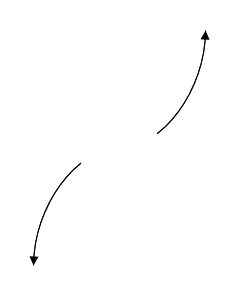
\includegraphics[width=0.3\textwidth]{../Figures/polyEndBehaviorDC.png}
    \end{center}\begin{enumerate}[label=\Alph*.]
\begin{multicols}{2}
\item 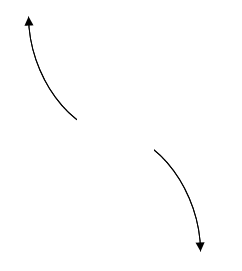
\includegraphics[width = 0.3\textwidth]{../Figures/polyEndBehaviorAC.png}
\item 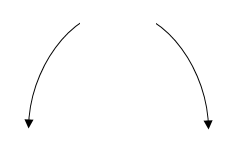
\includegraphics[width = 0.3\textwidth]{../Figures/polyEndBehaviorBC.png}
\item 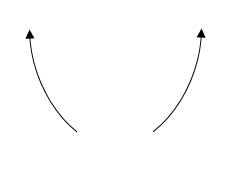
\includegraphics[width = 0.3\textwidth]{../Figures/polyEndBehaviorCC.png}
\item 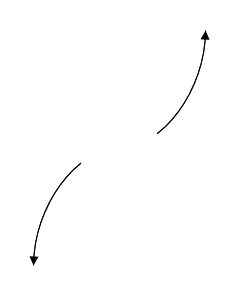
\includegraphics[width = 0.3\textwidth]{../Figures/polyEndBehaviorDC.png}
\end{multicols}\item None of the above.\end{enumerate}
\textbf{General Comment:} Remember that end behavior is determined by the leading coefficient AND whether the \textbf{sum} of the multiplicities is positive or negative.
}
\litem{
Describe the end behavior of the polynomial below.
\[ f(x) = 4(x + 3)^{2}(x - 3)^{7}(x + 8)^{5}(x - 8)^{6} \]The solution is the graph below, which is option C.
    \begin{center}
        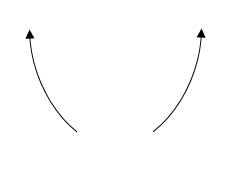
\includegraphics[width=0.3\textwidth]{../Figures/polyEndBehaviorCopyCC.png}
    \end{center}\begin{enumerate}[label=\Alph*.]
\begin{multicols}{2}
\item \includegraphics[width = 0.3\textwidth]{../Figures/polyEndBehaviorCopyAC.png}
\item \includegraphics[width = 0.3\textwidth]{../Figures/polyEndBehaviorCopyBC.png}
\item \includegraphics[width = 0.3\textwidth]{../Figures/polyEndBehaviorCopyCC.png}
\item \includegraphics[width = 0.3\textwidth]{../Figures/polyEndBehaviorCopyDC.png}
\end{multicols}\item None of the above.\end{enumerate}
\textbf{General Comment:} Remember that end behavior is determined by the leading coefficient AND whether the \textbf{sum} of the multiplicities is positive or negative.
}
\litem{
Construct the lowest-degree polynomial given the zeros below. Then, choose the intervals that contain the coefficients of the polynomial in the form $ax^3+bx^2+cx+d$.
\[ \frac{-3}{4}, -7, \text{ and } \frac{-1}{3} \]The solution is \( 12x^{3} +97 x^{2} +94 x + 21 \), which is option A.\begin{enumerate}[label=\Alph*.]
\item \( a \in [12, 14], b \in [94, 98], c \in [90, 105], \text{ and } d \in [20, 26] \)

* $12x^{3} +97 x^{2} +94 x + 21$, which is the correct option.
\item \( a \in [12, 14], b \in [-99, -94], c \in [90, 105], \text{ and } d \in [-26, -20] \)

$12x^{3} -97 x^{2} +94 x -21$, which corresponds to multiplying out $(4x -3)(x -7)(3x -1)$.
\item \( a \in [12, 14], b \in [-93, -88], c \in [31, 33], \text{ and } d \in [20, 26] \)

$12x^{3} -89 x^{2} +32 x + 21$, which corresponds to multiplying out $(4x -3)(x -7)(3x + 1)$.
\item \( a \in [12, 14], b \in [78, 86], c \in [-43, -37], \text{ and } d \in [-26, -20] \)

$12x^{3} +79 x^{2} -38 x -21$, which corresponds to multiplying out $(4x -3)(x + 7)(3x + 1)$.
\item \( a \in [12, 14], b \in [94, 98], c \in [90, 105], \text{ and } d \in [-26, -20] \)

$12x^{3} +97 x^{2} +94 x -21$, which corresponds to multiplying everything correctly except the constant term.
\end{enumerate}

\textbf{General Comment:} To construct the lowest-degree polynomial, you want to multiply out $(4x + 3)(x + 7)(3x + 1)$
}
\litem{
Describe the zero behavior of the zero $x = -9$ of the polynomial below.
\[ f(x) = 2(x - 4)^{10}(x + 4)^{6}(x + 9)^{10}(x - 9)^{7} \]The solution is the graph below, which is option B.
    \begin{center}
        \includegraphics[width=0.3\textwidth]{../Figures/polyZeroBehaviorBC.png}
    \end{center}\begin{enumerate}[label=\Alph*.]
\begin{multicols}{2}
\item \includegraphics[width = 0.3\textwidth]{../Figures/polyZeroBehaviorAC.png}
\item \includegraphics[width = 0.3\textwidth]{../Figures/polyZeroBehaviorBC.png}
\item \includegraphics[width = 0.3\textwidth]{../Figures/polyZeroBehaviorCC.png}
\item \includegraphics[width = 0.3\textwidth]{../Figures/polyZeroBehaviorDC.png}
\end{multicols}\item None of the above.\end{enumerate}
\textbf{General Comment:} You will need to sketch the entire graph, then zoom in on the zero the question asks about.
}
\litem{
Which of the following equations \textit{could} be of the graph presented below?

\begin{center}
    \includegraphics[width=0.5\textwidth]{../Figures/polyGraphToFunctionC.png}
\end{center}


The solution is \( 6(x + 4)^{4} (x - 2)^{8} (x + 3)^{7} \), which is option E.\begin{enumerate}[label=\Alph*.]
\item \( 15(x + 4)^{6} (x - 2)^{7} (x + 3)^{5} \)

The factor $(x - 2)$ should have an even power.
\item \( -6(x + 4)^{10} (x - 2)^{6} (x + 3)^{8} \)

The factor $(x + 3)$ should have an odd power and the leading coefficient should be the opposite sign.
\item \( 17(x + 4)^{10} (x - 2)^{7} (x + 3)^{10} \)

The factor $(x - 2)$ should have an even power and the factor $(x + 3)$ should have an odd power.
\item \( -19(x + 4)^{8} (x - 2)^{8} (x + 3)^{7} \)

This corresponds to the leading coefficient being the opposite value than it should be.
\item \( 6(x + 4)^{4} (x - 2)^{8} (x + 3)^{7} \)

* This is the correct option.
\end{enumerate}

\textbf{General Comment:} General Comments: Draw the x-axis to determine which zeros are touching (and so have even multiplicity) or cross (and have odd multiplicity).
}
\litem{
Construct the lowest-degree polynomial given the zeros below. Then, choose the intervals that contain the coefficients of the polynomial in the form $x^3+bx^2+cx+d$.
\[ 2 + 3 i \text{ and } 1 \]The solution is \( x^{3} -5 x^{2} +17 x -13 \), which is option B.\begin{enumerate}[label=\Alph*.]
\item \( b \in [-1.8, 1.9], c \in [-4.15, -3.21], \text{ and } d \in [2.99, 3.53] \)

$x^{3} + x^{2} -4 x + 3$, which corresponds to multiplying out $(x -3)(x -1)$.
\item \( b \in [-9.1, -3.5], c \in [16.78, 18.65], \text{ and } d \in [-14.03, -11.89] \)

* $x^{3} -5 x^{2} +17 x -13$, which is the correct option.
\item \( b \in [4.7, 5.3], c \in [16.78, 18.65], \text{ and } d \in [11.64, 13.41] \)

$x^{3} +5 x^{2} +17 x + 13$, which corresponds to multiplying out $(x-(2 + 3 i))(x-(2 - 3 i))(x + 1)$.
\item \( b \in [-1.8, 1.9], c \in [-3.38, -1.37], \text{ and } d \in [1.75, 2.85] \)

$x^{3} + x^{2} -3 x + 2$, which corresponds to multiplying out $(x -2)(x -1)$.
\item \( \text{None of the above.} \)

This corresponds to making an unanticipated error or not understanding how to use nonreal complex numbers to create the lowest-degree polynomial. If you chose this and are not sure what you did wrong, please contact the coordinator for help.
\end{enumerate}

\textbf{General Comment:} Remember that the conjugate of $a+bi$ is $a-bi$. Since these zeros always come in pairs, we need to multiply out $(x-(2 + 3 i))(x-(2 - 3 i))(x-(1))$.
}
\litem{
Describe the zero behavior of the zero $x = -4$ of the polynomial below.
\[ f(x) = 6(x - 4)^{7}(x + 4)^{12}(x + 3)^{4}(x - 3)^{6} \]The solution is the graph below, which is option B.
    \begin{center}
        \includegraphics[width=0.3\textwidth]{../Figures/polyZeroBehaviorCopyBC.png}
    \end{center}\begin{enumerate}[label=\Alph*.]
\begin{multicols}{2}
\item \includegraphics[width = 0.3\textwidth]{../Figures/polyZeroBehaviorCopyAC.png}
\item \includegraphics[width = 0.3\textwidth]{../Figures/polyZeroBehaviorCopyBC.png}
\item \includegraphics[width = 0.3\textwidth]{../Figures/polyZeroBehaviorCopyCC.png}
\item \includegraphics[width = 0.3\textwidth]{../Figures/polyZeroBehaviorCopyDC.png}
\end{multicols}\item None of the above.\end{enumerate}
\textbf{General Comment:} You will need to sketch the entire graph, then zoom in on the zero the question asks about.
}
\litem{
Construct the lowest-degree polynomial given the zeros below. Then, choose the intervals that contain the coefficients of the polynomial in the form $ax^3+bx^2+cx+d$.
\[ \frac{1}{2}, \frac{5}{4}, \text{ and } \frac{-1}{5} \]The solution is \( 40x^{3} -62 x^{2} +11 x + 5 \), which is option A.\begin{enumerate}[label=\Alph*.]
\item \( a \in [37, 43], b \in [-63, -59], c \in [10, 12], \text{ and } d \in [4, 9] \)

* $40x^{3} -62 x^{2} +11 x + 5$, which is the correct option.
\item \( a \in [37, 43], b \in [-24, -15], c \in [-38, -26], \text{ and } d \in [-12, -4] \)

$40x^{3} -22 x^{2} -31 x -5$, which corresponds to multiplying out $(2x + 1)(4x -5)(5x + 1)$.
\item \( a \in [37, 43], b \in [-63, -59], c \in [10, 12], \text{ and } d \in [-12, -4] \)

$40x^{3} -62 x^{2} +11 x -5$, which corresponds to multiplying everything correctly except the constant term.
\item \( a \in [37, 43], b \in [74, 85], c \in [38, 41], \text{ and } d \in [4, 9] \)

$40x^{3} +78 x^{2} +39 x + 5$, which corresponds to multiplying out $(2x + 1)(4x + 5)(5x + 1)$.
\item \( a \in [37, 43], b \in [55, 66], c \in [10, 12], \text{ and } d \in [-12, -4] \)

$40x^{3} +62 x^{2} +11 x -5$, which corresponds to multiplying out $(2x + 1)(4x + 5)(5x -1)$.
\end{enumerate}

\textbf{General Comment:} To construct the lowest-degree polynomial, you want to multiply out $(2x -1)(4x -5)(5x + 1)$
}
\litem{
Which of the following equations \textit{could} be of the graph presented below?

\begin{center}
    \includegraphics[width=0.5\textwidth]{../Figures/polyGraphToFunctionCopyC.png}
\end{center}


The solution is \( 4x^{4} (x - 1)^{11} (x + 2)^{11} \), which is option D.\begin{enumerate}[label=\Alph*.]
\item \( -2x^{8} (x - 1)^{5} (x + 2)^{7} \)

This corresponds to the leading coefficient being the opposite value than it should be.
\item \( 13x^{9} (x - 1)^{4} (x + 2)^{9} \)

The factor $0$ should have an even power and the factor $1$ should have an odd power.
\item \( -14x^{8} (x - 1)^{7} (x + 2)^{10} \)

The factor $(x + 2)$ should have an odd power and the leading coefficient should be the opposite sign.
\item \( 4x^{4} (x - 1)^{11} (x + 2)^{11} \)

* This is the correct option.
\item \( 7x^{8} (x - 1)^{6} (x + 2)^{7} \)

The factor $(x - 1)$ should have an odd power.
\end{enumerate}

\textbf{General Comment:} General Comments: Draw the x-axis to determine which zeros are touching (and so have even multiplicity) or cross (and have odd multiplicity).
}
\end{enumerate}

\end{document}